\chapter{Analýza}
Tato kapitola je zaměřena na představení aktuálně používaných multiplatformních frameworků a porovnání těchto frameworků
s technologií Compose Multiplatform. Shrnuje jejich podstatné rysy a následně slouží k
jednoduššímu porovnání a vyhodnocení použitelnosti frameworku Compose Multiplatform. Zároveň je v této kapitole detailněji
rozebrán samotný Compose Multiplatform a jak z pohledu implementace uživatelského rozhraní, tak i z pohledu implementace
aplikační logiky, ke které využívá technologii Kotlin Multiplatform.

Po dokončení analýzy obou těchto technologií se práce věnuje porovnáním všech těchto frameworků jednak z pohledu architektury
a náročnosti implementace, tak z pohledu výkonu aplikací implementovaných pomocí těchto technologií. 

Konec této kapitoly je věnován limitacím frameworku Compose Multiplatform oproti nativním řešením, které přímo vyplývají 
z provedené analýzy.  


\section{Přehled existujících frameworků}
Mezi aktuálně nejpopulárnější multiplatformní frameworky jednoznačně patří Flutter a React Native. \cite{crossPlatformFrameworksStats}
V následujících kapitolách jsou proto tyto nejpoužívanější frameworky podrobně porovnány s frameworkem Compose Multiplatform a u každého z nich 
jsou vybrány důležité vlastnosti, které jsou pro tyto frameworky typické. 

Jednotlivé frameworky jsou seřazeny postupně od nejstaršího
po nejmladší, což umožňuje lepší náhled na to, jak se jednotlivé frameworky vyvíjely v čase. Pro lepší ilustraci rozdílů 
mezi jednotlivými frameworky byla zvolena 
podobná struktura jednotlivých kapitol, čehož bylo možné docílit díky mnoha společnými rysům napříč frameworky.

%---------------------------------------------------------------
\subsection{React Native}
%---------------------------------------------------------------
React Native byl jedním z prvních frameworků pro tvorbu multiplatformního UI a do jisté míry ovlivnil i ostatní popisované
frameworky. Jeho vývoj započal ve společnosti Facebook během interního hackaton projektu a první jeho oficiálně publikovaná
verze vyšla začátkem roku 2015. \cite{reactNativeHistory}
Nyní se jedná o open-source framework, kde jeho hlavním cílem je umožnit vývojářům vytvářet nativní mobilní aplikace 
pro platformy Android a iOS z jednoho společného kódu napsaného v jazyce JavaScript nebo TypeScript.

\section*{Klíčové vlastnosti React Native}

\myparagraph{Komponentní architektura} 
React Native využívá komponentní architekturu, která vývojářům umožňuje 
vytvářet znovupoužitelné komponenty. \cite{reactNativeComponents} Tato architektura je jednak založena na obecných
React komponentách, ale zároveň také na React Native specifických komponentách, které se dále dělí na takzvané core
komponenty, komponenty vytvořené komunitou či vlastní nativní komponenty. \cite{reactNativeComponents}

% // todo komponenty prekladane na nativni 
    
\myparagraph{Deklarativní zápis UI}
React Native stejně jako React pro webové aplikace využívá pro zápis UI deklarativní způsob, 
při kterém využívá JSX (JavaScript XML) syntaxe k popisu struktury UI komponent. \cite{reactNativeJSX}
Takto zapsané UI lépe reflektovalo aktuální stav aplikace.
Tento způsob zápisu začal na mobilních platformách růst popularitě právě díky Reactu Native, který po svém uvolnění v roce 2013 
defacto nastartoval éru deklarativního zápisu UI na mobilních platformách. \cite{declarativeUIHistory}

\myparagraph{Fast Refresh} 
Fast Refresh je v funkce, která vývojářům umožňuje okamžitě vidět výsledky provedených 
změn v kódu bez nutnosti znovu sestavení aplikace. \cite{reactNativeFastRefresh}

\myparagraph{JavaScript/TypeScript} 
Aplikační logika v React Native se píše v jazyce JavaScript nebo TypeScript, 
což usnadňuje snadnou integraci s existujícími webovými technologiemi. \cite{reactNativeFundamentals}

\myparagraph{Rozsáhlá komunita} 
React Native má rozsáhlou komunitu vývojářů, což vede k bohatému ekosystému 
třetích stran, včetně mnoha dostupných knihoven a modulů. \cite{reactNativeComunity}

\myparagraph{Expo framework} 
Pro ještě snazší start vývoje poskytuje React Native Expo framework, který 
zjednodušuje proces vývoje a umožňuje rychlé prototypování. \cite{reactNativeExpo}

\subsection*{Architektura frameworku React Native}

React native do roku 2022 využíval architekturu založenou na návrhového vzoru Bridge, který spojoval kód napsaný v JavaScriptu s nativní kódem určeným pro danou platformu. 
Tyto dva celky byly spuštěny na souběžných vláknech a komunikovaly spolu pomocí zasílání serializovaných zpráv. Časem se ale ukázalo, že se tato komunikace
a další její charakteristiky stávají úzkým hrdlem celého systému a byla proto od verze 0.68 nahrazena JavaScriptovým rozhraním zvaným JSI. \cite{reactNativeAboutNewArch}

JSI nově JavaScriptu umožňuje držet referenci na C++ objekty a volat nad nimi potřebné metody. \cite{reactNativeAboutNewArch} Toho využívá nový renderovací systém zvaný \textit{Fabric}, který 
frameworku napomáhá sjednotit renderovací logiku prováděnou v C++ a zlepšit tak interoperabilitu s nativními platformami.

\begin{figure}[H]
  \centering
  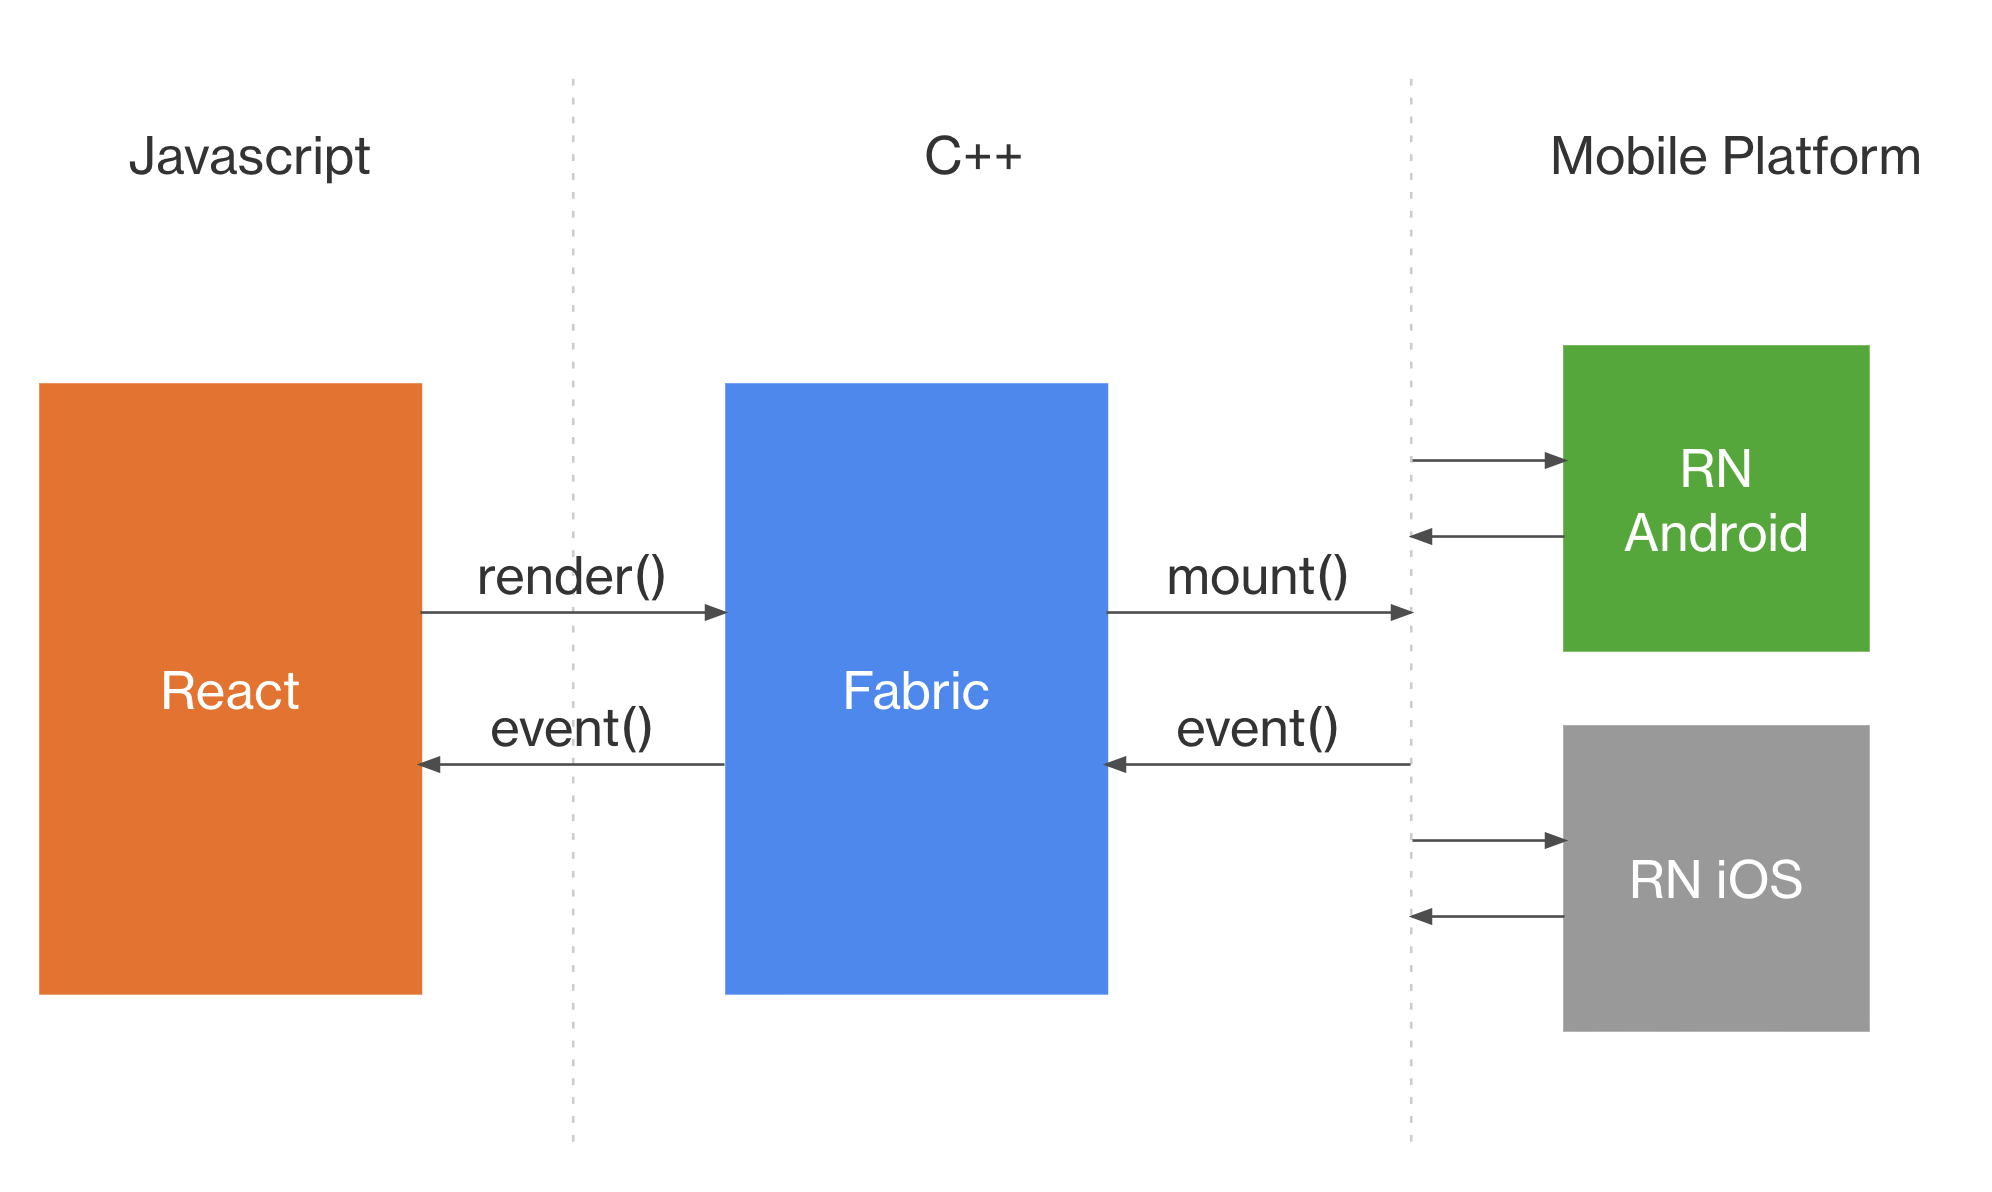
\includegraphics[width=0.85\textwidth]{react-natice-xplat-implementation-diagram.png}
  \caption{React Native }
  \label{fig:react-natice-xplat-implementation-diagram}
\end{figure}

% \begin{figure}[H]
%   \centering
%   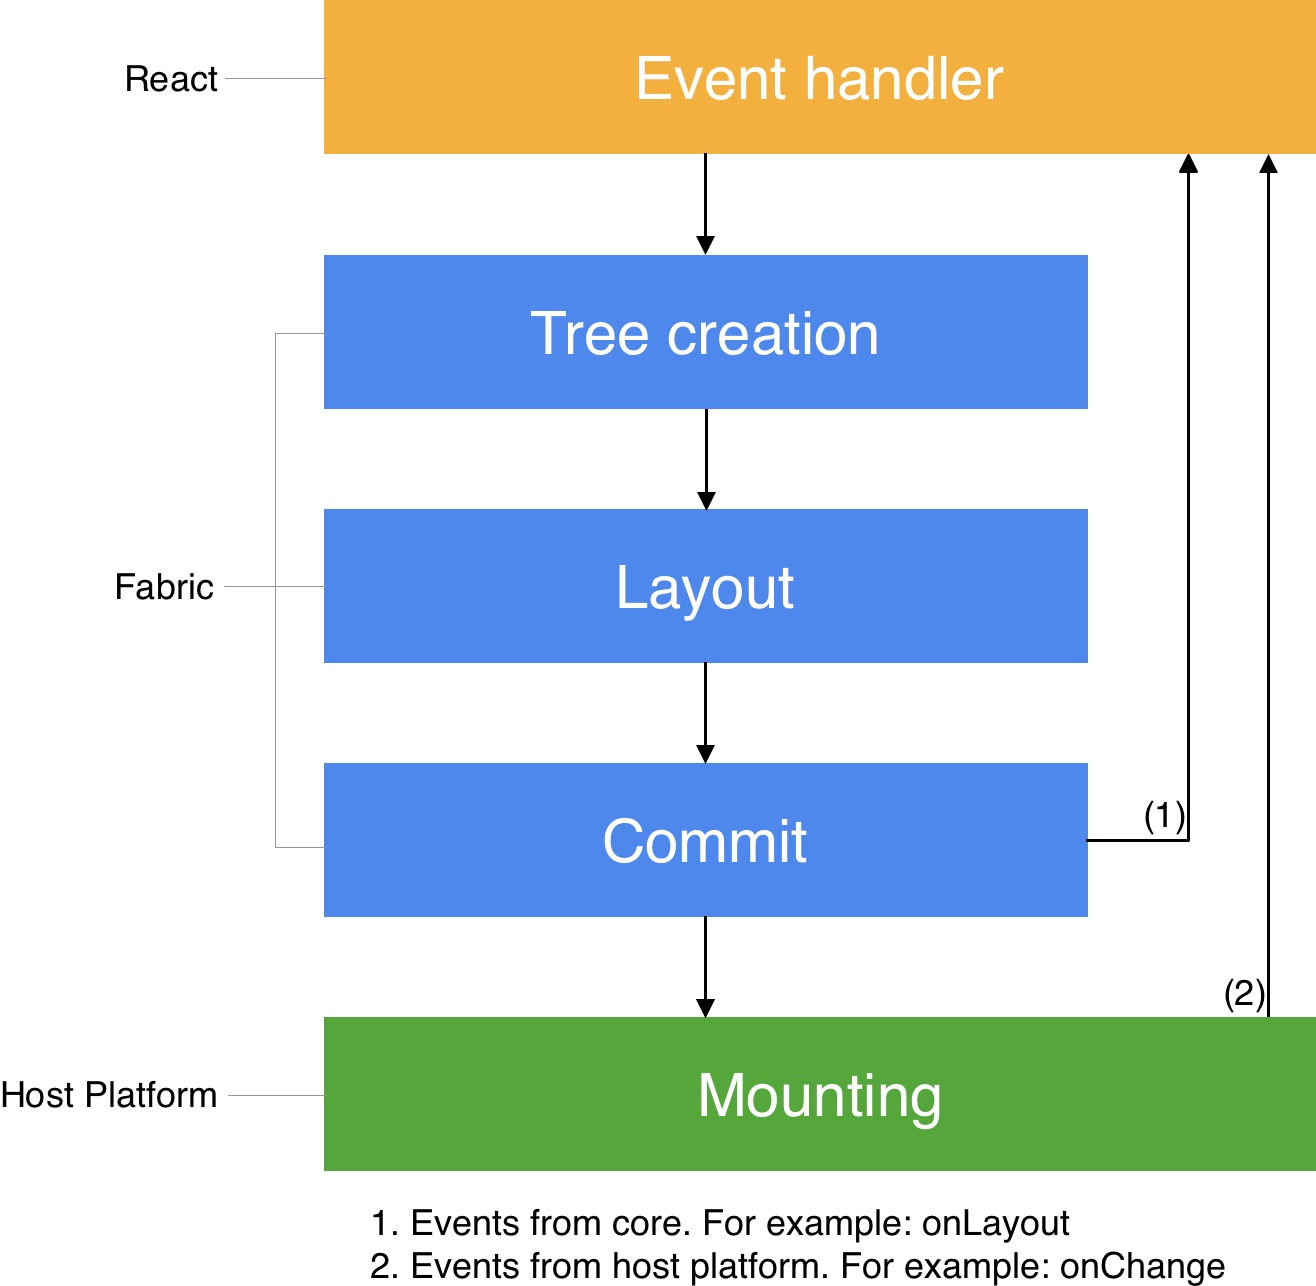
\includegraphics[width=0.55\textwidth]{react-native-data-flow.jpg}
%   \caption{React Native tok dat}
%   \label{fig:react-natice-data-flow}
% \end{figure}


% I přes tyto změny React Native stále využívá systém dvou typů vláken označovaných jako \textit{JavaScript Thread} a \textit{UI Thread} (známé taktéž pod názvem \textit{Main Thread}) 
% mezi které rozděluje práci.


Jak je vidět na obrázku \ref{fig:react-natice-xplat-implementation-diagram}, tak \textit{Fabric} de facto plní funkci prostředníka, který převádí React 
komponenty na nativní komponenty pro každou platformu. 

Pro lepší představu jak dané komponenty vypadají slouží následující ukázka kódu \ref{lst:reactNativeJSX}.

\begin{listing}[H]
\caption{Popis UI komponent pomoci JSX}\label{lst:reactNativeJSX}
\begin{minted}{jsx}
    function MyComponent() {
      return (
        <View>
          <View
            style={{backgroundColor: 'red', height: 20, width: 20}}
          />
          <View
            style={{backgroundColor: 'blue', height: 20, width: 20}}
          />
        </View>
      );
    }
    // <MyComponent />
\end{minted}
\end{listing}




Na ukázce kódu \ref{lst:reactNativeJSX} jsou použity některé z nejpoužívanějších core komponent, které se při psaní React
Native aplikací používají. \cite{reactNativeComponents} Jak již bylo zmíněno dříve, tak tyto komponenty jsou následně převedeny 
na nativní komponenty pro každou platformu a to jakým způsobem Fabric dané komponenty převádí se dá rozdělit do následujících tří
na sebe navazujících fází: \cite{reactNativeRenderCommitMount}
 
%Na této ukázce je zároveň vidět použití deklarativního zápisu, které bude podrobněji probráno v následující kapitole.

\smallskip

\myparagraph{Render}
Během této fáze se z jednotlivých komponent (React Elementů) sestaví strom elementů v JavaScriptu (viz levá část obrázku \ref{fig:react-native-render-pipeline}) a nad tímto stromem se 
následně spustí rekurzivní redukce, při které dojde k vytvoření nového stromu takzvaného React Shadow Tree. (viz prostřední část obrázku \ref{fig:react-native-render-pipeline})
\cite{reactNativeRenderCommitMount} Ten se skládá z jednotlivých React Shadow Nodes, které reprezentují objekty v C++ a tím přechází tato renderovací fáze do další fáze zvané commit.\cite{reactNativeRenderCommitMount}

\myparagraph{Commit}
V rámci této fáze je pro každý React Shadow Node vypočítána jeho pozice a velikost na koncovém zařízení a díky tomu může renderovací systém
přejít k poslední fázi zvané Mount. \cite{reactNativeRenderCommitMount}

\myparagraph{Mount}
Během této poslední fáze dojde k transformaci \textit{React Shadow Tree} na \textit{Host View Tree} (viz pravá část obrázku \ref{fig:react-native-render-pipeline}) a to tak, že každý \textit{React Shadow Node}
se transformuje na jeho ekvivalent v nativní podobě. \cite{reactNativeRenderCommitMount} Čili například na platformě Android se $<ViewShadowNode>$ přetransformuje na android.view.ViewGroup. \cite{reactNativeRenderCommitMount}

\begin{figure}[H]
  \centering
  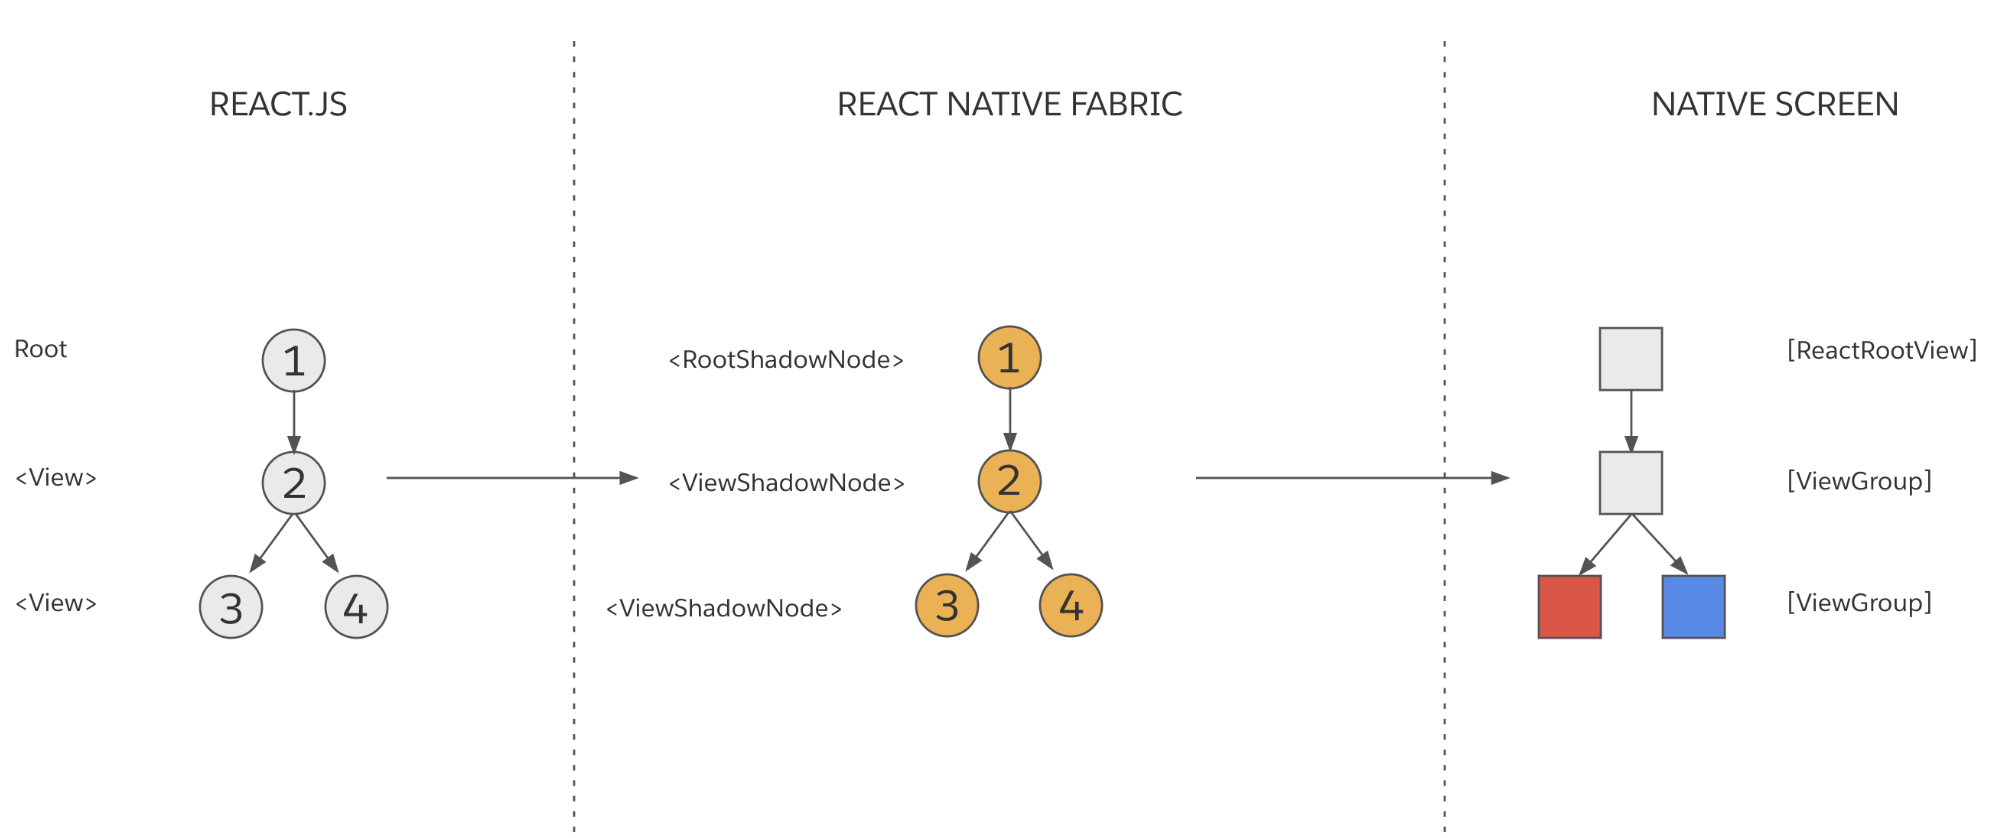
\includegraphics[width=0.99\textwidth]{react-native-render-pipeline.png}
  \caption{React Native vykreslovací fáze}
  \label{fig:react-native-render-pipeline}
\end{figure}

%---------------------------------------------------------------
\subsection{Flutter}
%---------------------------------------------------------------
Flutter je open-source softwarový toolkit pro vývoj uživatelských rozhraní (UI). \cite{flutterfaq} Za vývojem stojí společnost Google a je určený k vytváření nativně kompilovaných 
aplikací pro mobilní zařízení, web a desktop z jednoho zdrojového kódu. \cite{flutterfaq}
Byl vydán v roce 2017 a získal značnou popularitu mezi vývojáři díky svému snadnému použití, flexibilitě a schopnostem tvorby UI.

\subsection*{Klíčové vlastnosti Flutteru}

\myparagraph{UI založené na widgetech} 
Flutter využívá reaktivně deklarativní UI založené na widgetech. \cite{flutterUI} Widgety jsou základními stavebními 
bloky Flutter aplikací, představující vše od strukturálních prvků po stylistické komponenty. \cite{flutterWidgets}

\myparagraph{Hot Reload} 
Další z významných funkcí Flutteru, která významně zrychluje vývojový proces a zvyšuje produktivitu je funkce "Hot Reload". 
Během vývoje běží Flutter aplikace na virtuálním počítači (Dart VM), který díky této funkci umožňuje okamžitě vidět provedené změny
v kódu bez nutnosti úplné rekompilace aplikace. \cite{flutterHotReload} Teprve pro vydání jsou Flutter aplikace kompilovány přímo do strojového kódu, 
ať už jde o instrukce Intel x64 nebo ARM, případně do JavaScriptu pokud jsou cíleny na web. \cite{flutterArchOverview}


\myparagraph{Jeden zdrojový kód pro více platforem} 
S Flutterem mohou vývojáři psát jeden zdrojový kód pro obě platformy Android a iOS, což snižuje dobu vývoje a úsilí 
vynakládané na údržbu. Flutter také rozšířil svou podporu pro cílení webových a desktopových aplikací, umožňující širší dosah s minimálními změnami kódu. \cite{flutter}

\myparagraph{Rozsáhlá sada widgetů}
Flutter poskytuje komplexní sadu přizpůsobitelných widgetů, které usnadňují vytváření složitých a vizuálně 
atraktivních uživatelských rozhraní. Tyto widgety zahrnují vše od základních tlačítek a textových polí až po 
pokročilé komponenty jako jsou grafy a animace. \cite{flutterWidgets2}

\myparagraph{Programovací jazyk Dart}
Aplikace vytvořené pomocí frameworku Flutter jsou psány v jazyce Dart, moderním objektově orientovaném programovacím jazyce 
vyvinutém společností Google. Dart je navržen pro optimální výkon a produktivitu, což ho činí vhodným pro mobilní a
webový vývoj. \cite{dart}

\myparagraph{Způsob renderovaní UI}
Na rozdíl od Reactu Native Flutter nepoužívá platformě specifické komponenty koncových zařízení, ale veškeré UI komponenty (widgety)
renderuje pomocí vlastního renderovacího enginu. \cite{flutterRenderingModel}


\subsection*{Architektura frameworku Flutter} 
Jak je vidět na obrázku \ref{fig:flutter_architectural_layers}, tak architektura Flutteru je rozdělena do tří hlavních vrstev. \cite{flutterArchOverview}
Embedder je vrstva, která umožňuje integrovat Flutter do konkrétních platforem jako je Android, iOS, desktop nebo web. 
Každý embedder obsahuje platformě specifický kód, který je potřebný pro spuštění Flutteru na dané platformě.
Engine je vrstva starající se o vykreslování grafiky, kdykoli kdy je potřeba vykreslit nový snímek. \cite{flutterArchOverview} 
Framework je vrstva, která je používána vývojáři k vytváření uživatelských rozhraní a definování chování aplikace. 
Obsahuje hotové widgety, funkce pro manipulaci s UI a další nástroje pro vývojáře. \cite{flutterArchOverview} 


\begin{figure}[H]
  \centering
  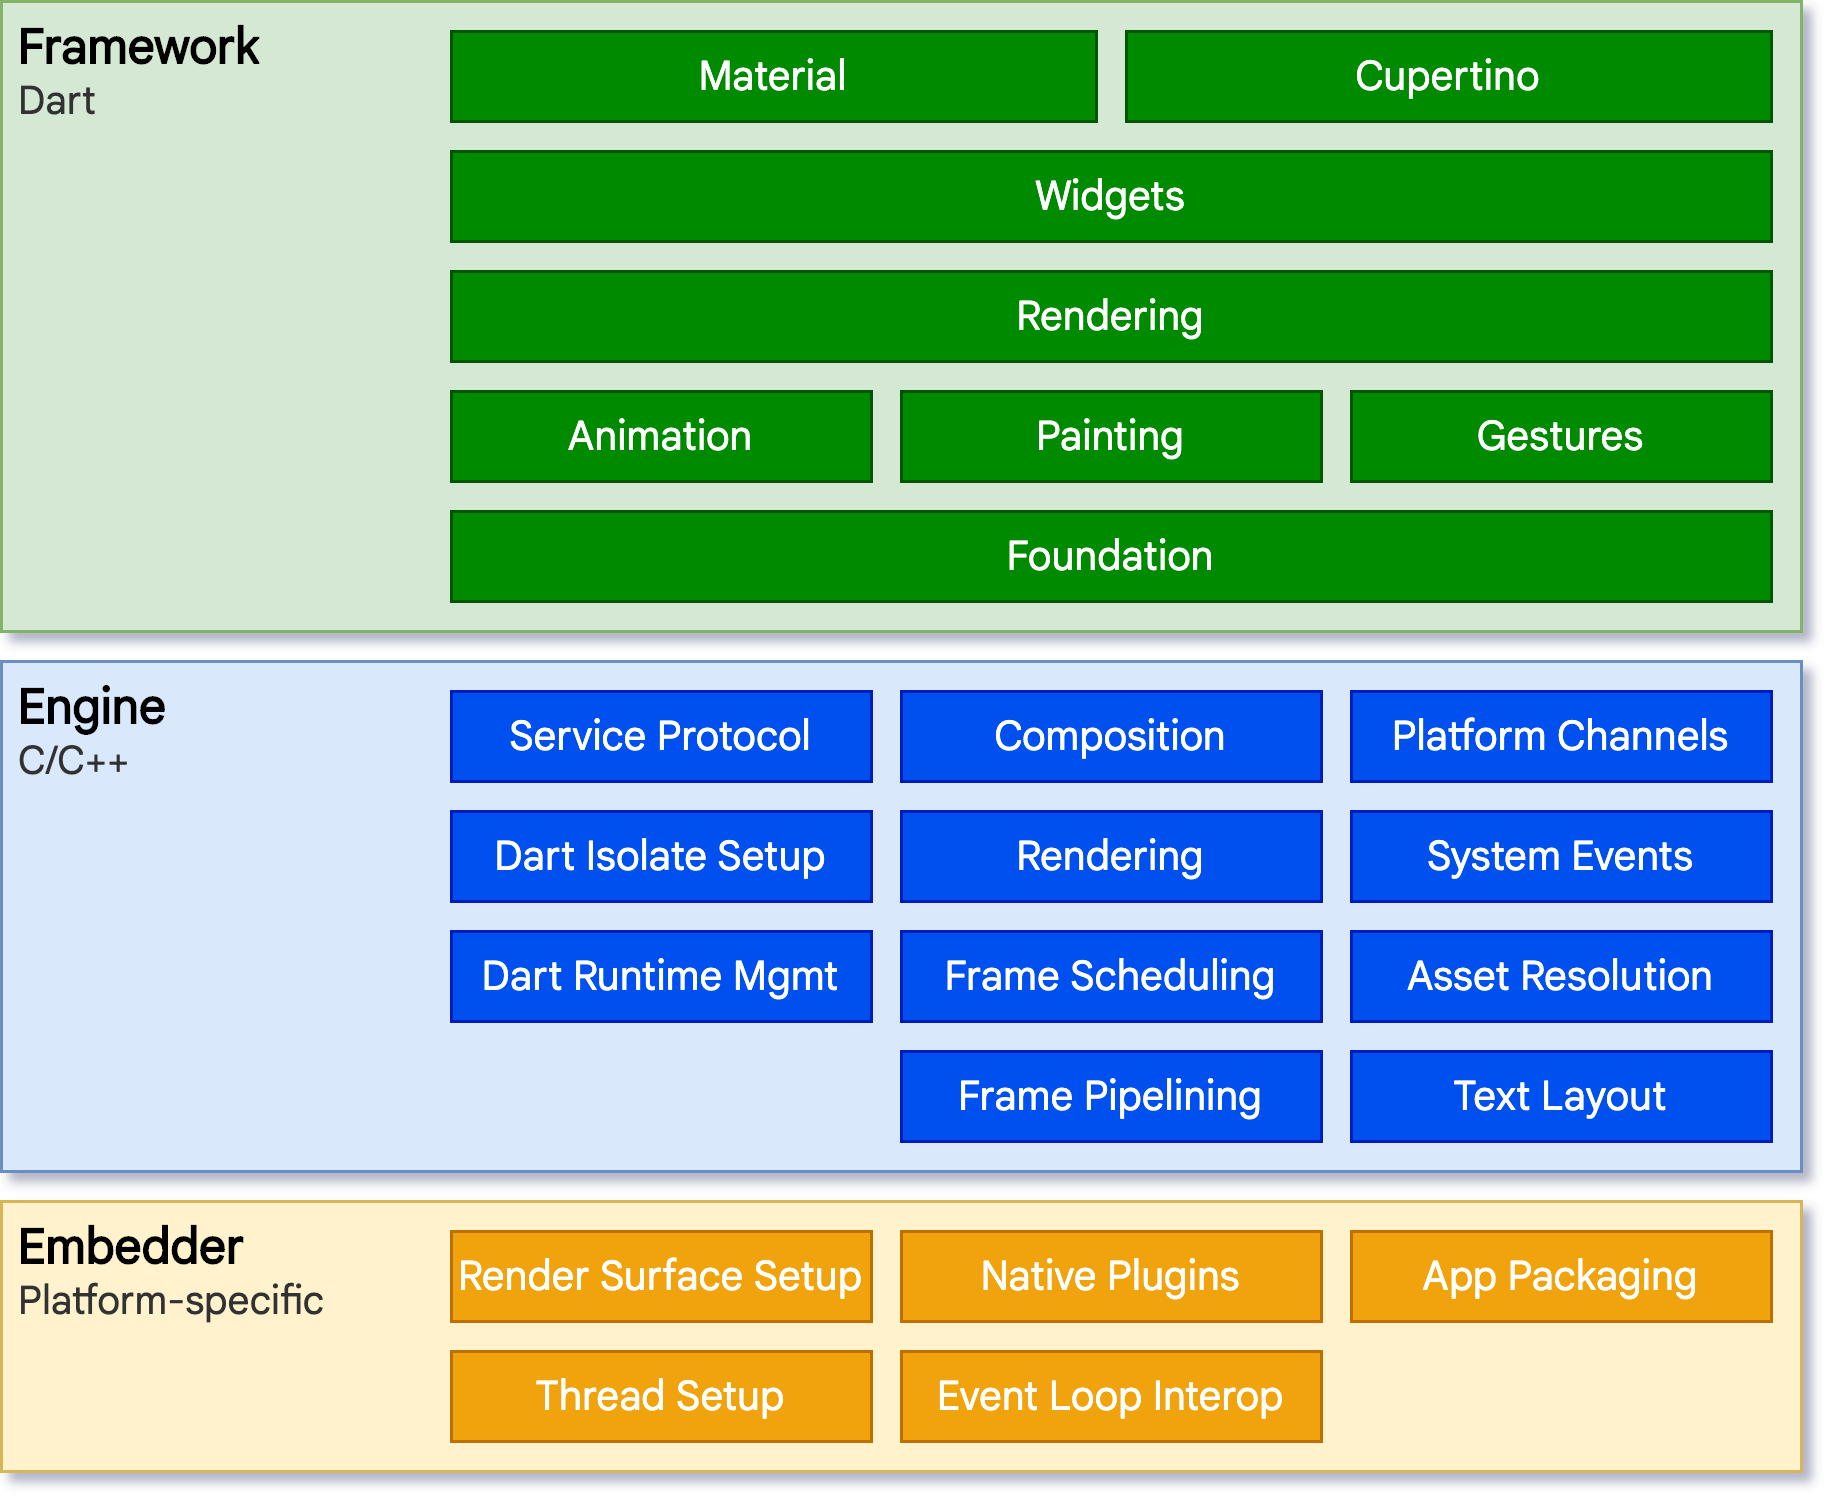
\includegraphics[width=0.85\textwidth]{flutter_architectural_layers.png}
  \caption{Flutter architectural layers}
  \label{fig:flutter_architectural_layers}
\end{figure}

Mezi hierarchicky poslední a neméně důležitou častí tohoto frameworku jsou platformě specifické knihovny Material and Cupertino. Tyto knihovny
jsou následně využívány widgety k implementaci konkrétního design systému. Díky tomu je možné uživateli navodit nativní pocit z dané aplikace.

\medskip

Z pohledu UI je důležitým prvkem právě Flutter framework, který zároveň definuje jak spolu jednotlivé widgety interagují.

Widget je ve Flutteru základní stavební blok pro tvorbu uživatelského rozhraní. \cite{flutterWidgets} V následující ukázce kódu \ref{lst:flutterCode} je pro příklad použito několik 
základních widgetů jako je \emph{Image} nebo \emph{Text} a taktéž layout widget zvaný \emph{Container} a \emph{Row} pro organizaci a 
rozložení vnořených widgetů na obrazovce.

\begin{listing}[H]
\caption{Popis UI widgetů pomocí jazyka Dart}\label{lst:flutterCode}
\begin{minted}{dart}
Container(
  color: Colors.blue,
  child: Row(
    children: [
      Image.network('https://www.example.com/1.png'),
      const Text('A'),
    ],
  ),
);
\end{minted}
\end{listing}

Když Flutter potřebuje vykreslit tento blok, zavolá metodu \emph{build()} a ta vrátí podstrom widgetů, které následně vykreslí uživatelské 
rozhraní na základě aktuálního stavu aplikace. \cite*{flutterArchOverview}

Během fáze sestavování překládá Flutter widgety vyjádřené v kódu (například kód \ref{lst:flutterCode}) do odpovídajícího stromu elementů viz obrázek \ref{fig:flutter_trees}, přičemž každý widget má jeden element a 
každý prvek představuje určitou instanci widgetu v daném umístění stromové hierarchie. \cite*{flutterArchOverview}


\begin{figure}[H]
  \centering
  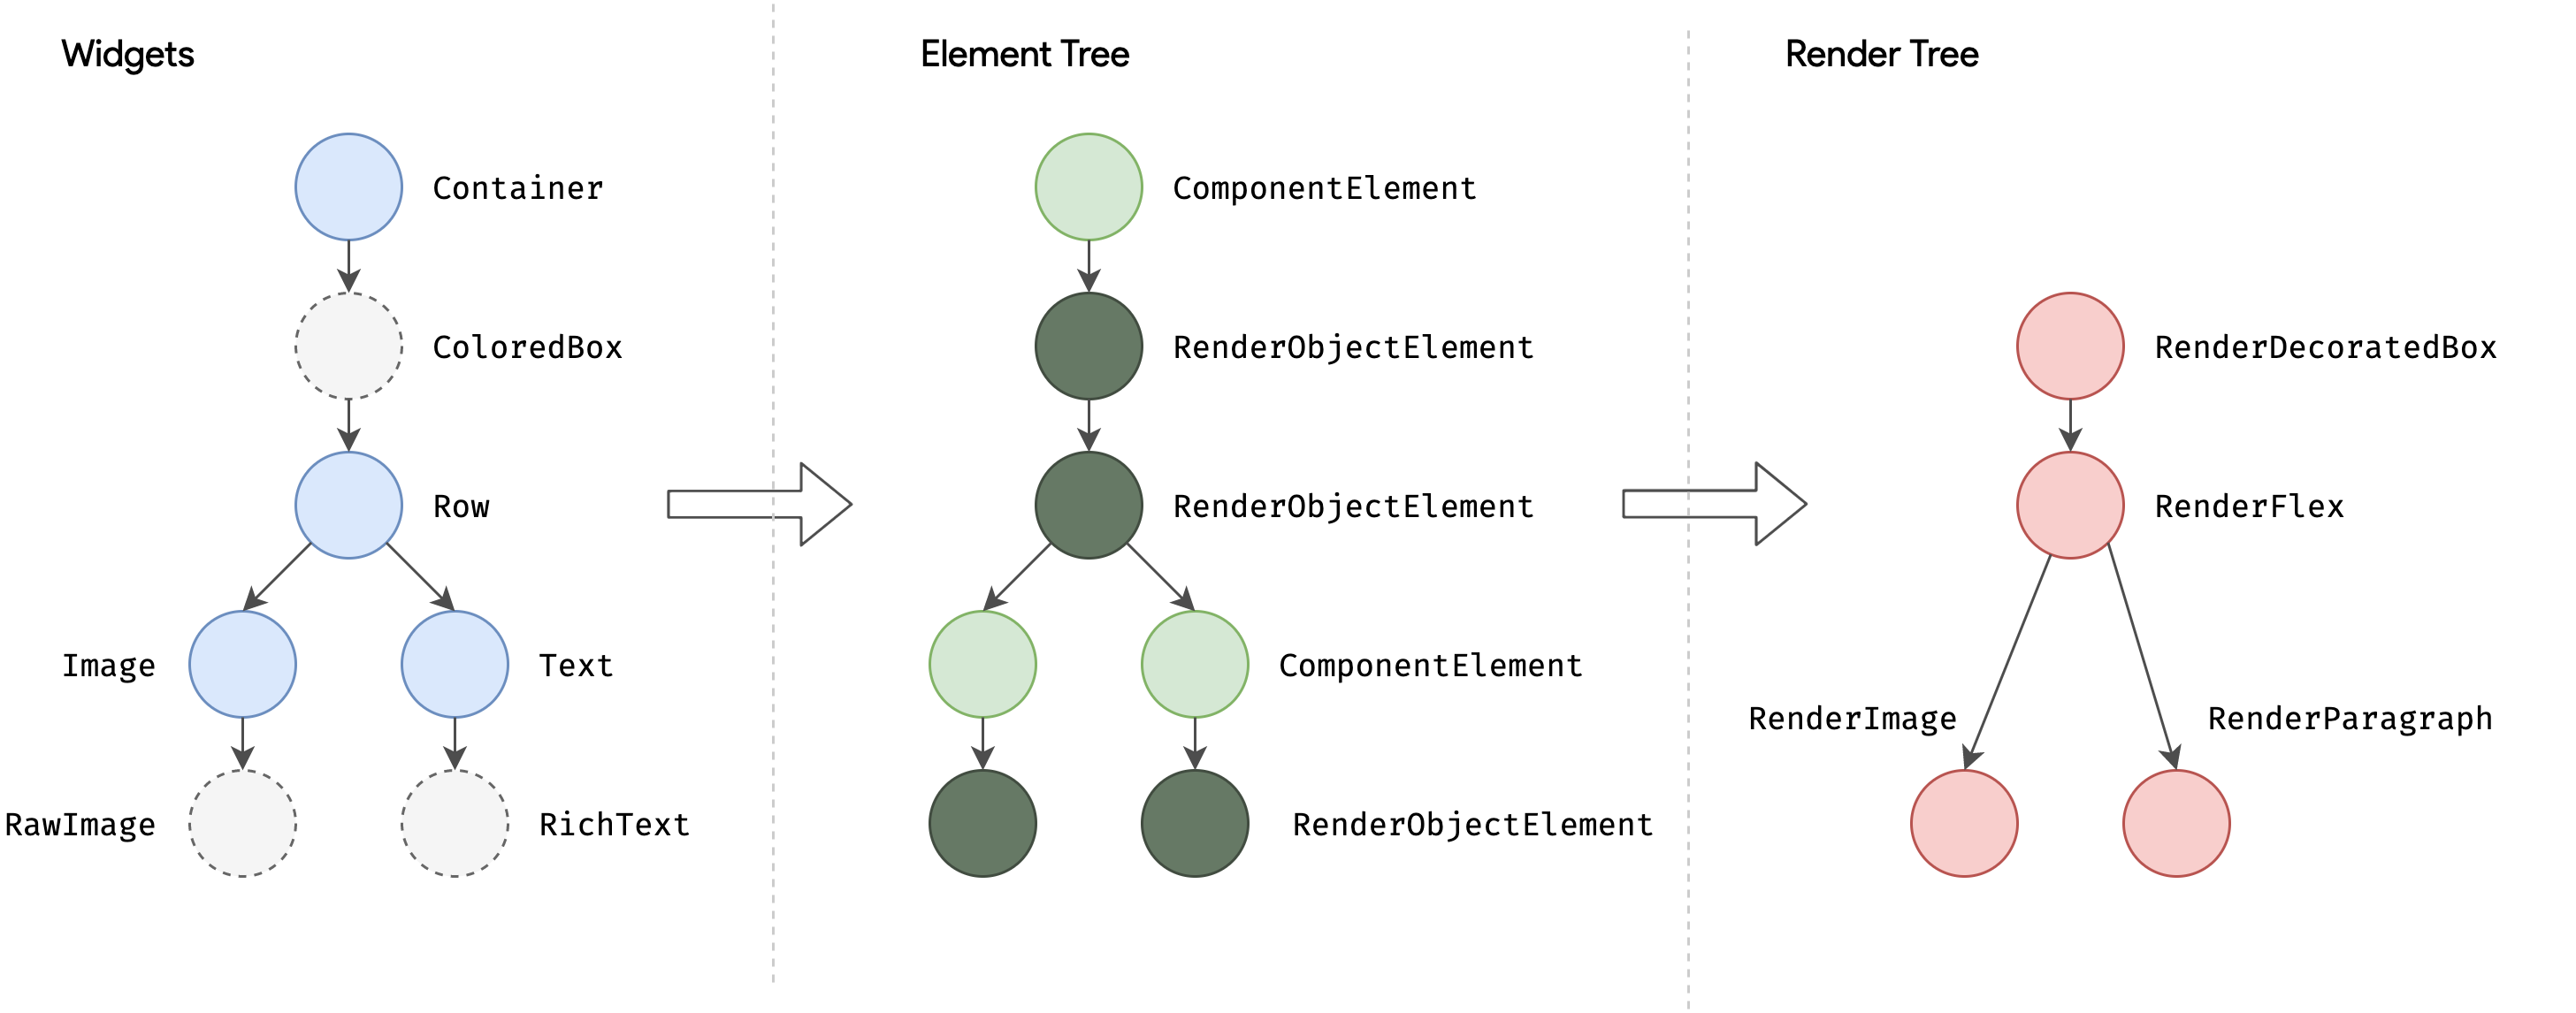
\includegraphics[width=1\textwidth]{flutter_trees.png}
  \caption{Flutter build proces}
  \label{fig:flutter_trees}
\end{figure}


\subsection{Compose Multiplatform}

Compose Multiplatform je framework sloužící k tvorbě uživatelských rozhraní použitelných na vícero platformách za 
jehož vývojem stojí společnost JetBrains. \cite{composeMultiplatform} Je založen na toolkitu zvaném Jetpack Compose, který je aktuálně 
doporučovaný k tvorbě nativních uživatelských rozhraních na platformě Android. \cite{jetpack}

Podporuje platformy jako Android, iOS (Alpha), Windows, MacOS, Linux a Web (experimentální). \cite{composeMultiplatform}

\medskip

\subsection*{Klíčové vlastnosti Compose Multiplatform}

\myparagraph{Deklarativní zápis UI} 
Používá deklarativní syntaxi pro popis uživatelského rozhraní. \cite{KMPUseCases}

\myparagraph{Jednotný kód pro různé platformy} 
Umožňuje sdílet kód pro Android, iOS, web i desktop. \cite{composeMultiplatform}

\myparagraph{Snadné migrace díky postupné integraci} 
Díky KMP je možné postupně implementovat jednotlivé částí aplikace i do již existujících aplikací s minimálním rizikem oproti
ostatním multiplatformním technologiím. \cite{KMP}

\myparagraph{Znovupoužitelnost Kotlin kódu} 
Díky KMP je možné použít některé části kódu z již existujících Android aplikací i na ostatních platformách.

\myparagraph{Programovací jazyk Kotlin} 
Frontendová i backendová část aplikace jsou psány v jazyce Kotlin pro bezproblémovou integraci se serverovou částí.

\myparagraph{Podpora od JetBrains}
Poskytuje stabilní podporu od vývojářského týmu JetBrains.

\subsection*{Architektura frameworku Compose Multiplatform} \label{ComposeArch}
Jelikož je framework Compose Multiplatform z velké části založen na frameworku Jetpack Compose, tak v této kapitole bude probírána
právě architektura toho frameworku, která bude doplněna o drobné rozdíly mezi těmito dvěma frameworky.

V porovnání s ostatními dříve zmíněnými frameworky slouží tento framework pouze k tvorbě multiplatformního UI a z toto důvodu je převážně 
používán s toolkitem Kotlin Multiplatform, který dané aplikaci poskytuje i multiplatformní aplikační logiku. Jelikož se jedná o základní 
komponentu bez které by Compose Multiplatform nevznikl, tak je tomuto toolkitu věnována celá kapitola \ref{kmpSection}.

Pro lepší ukázku toho, z jakých částí se typická multiplatformní mobilní aplikace skládá slouží následující obrázek \ref{fig:composeIOS}, který
vizualizuje propojenost frameworku Compsose Multiplatfom s toolkitem Kotlin Multiplatfom (KMP). Dále vizualizuje 
vztah platformě specifických knihoven pro tvorbu UI jako SwiftUI k frameworku Compose Multiplatform.
Compose Multiplatform lze nicméně použít i s technologiemi pro tvorbu UI jako je UI kit pro platformu iOS nebo
Android views  pro platformu Android, od kterých je postupně upouštěno a přechází se k deklarativním frameworkům jako je Jetpack Compose nebe SwiftUI.  

\begin{figure}[H]
  \centering
  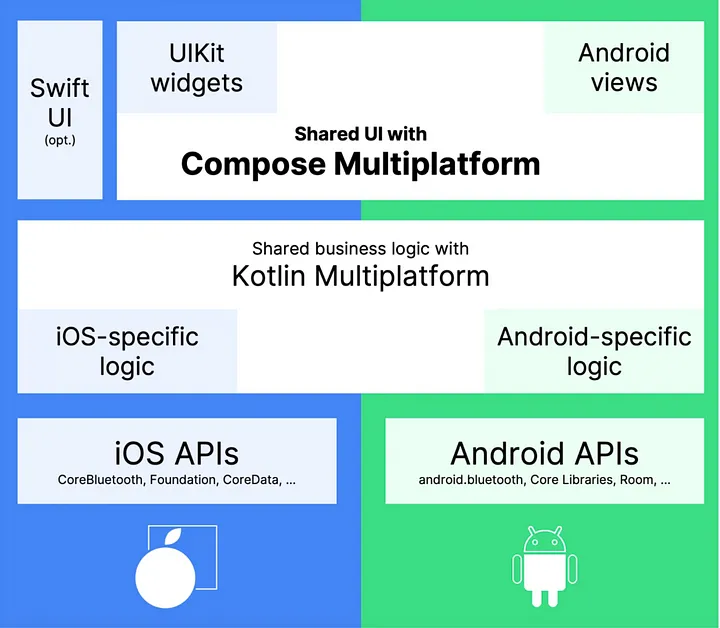
\includegraphics[width=.7\textwidth]{composeIOS.png}
  \caption{Compose Multiplatform iOS}
  \label{fig:composeIOS}
\end{figure}

TODO % doplnit neco o KMP a APIs

Co se týče samotného UI kódu, tak ten se skládá z jednotlivým funkcí označených anotací \code{@Composable}, která v těle obsahuje další
\textit{Composable} funkce (viz výpis kódu \ref{lst:ComposeCode}) jako jsou například \code{Column} pro strukturování vnořených elementů do sloupce nebo \code{Text} pro zobrazení
textu na obrazovce. 


\begin{listing}[H]
\caption{Popis UI widgetů pomocí jazyka Kotlin}\label{lst:ComposeCode}
\begin{minted}{kotlin}
@Composable
fun MyComposable() {
    Column {
        Text("Hello")
        Text("World")
    }
}
\end{minted}
\end{listing}

Takto strukturovaný kód může být následně frameworkem vykreslen na obrazovku k čemuž dochází v těchto třech následujících fázích:

\myparagraph{Composition}
Během této fáze Jetpack Compose vytvoří stromovou strukturu reprezentující UI komponenty, které mají být vykresleny.\cite{jetpackPhases} 
Tato stromová struktura je tvořena na základě do sebe zanořených Composable funkcí, které představují jednotlivé prvku uživatelského rozhraní.
Lepé tutu skutečnost reprezentuje obrázek \ref{fig:semantics-ui-tree}, na kterém je vidět, že nejspodnější vrstvu UI, reprezentuje kořenový uzel
sémantického stromu a následující vnořené prvky jsou jeho potomky.

\begin{figure}[H]
  \centering
  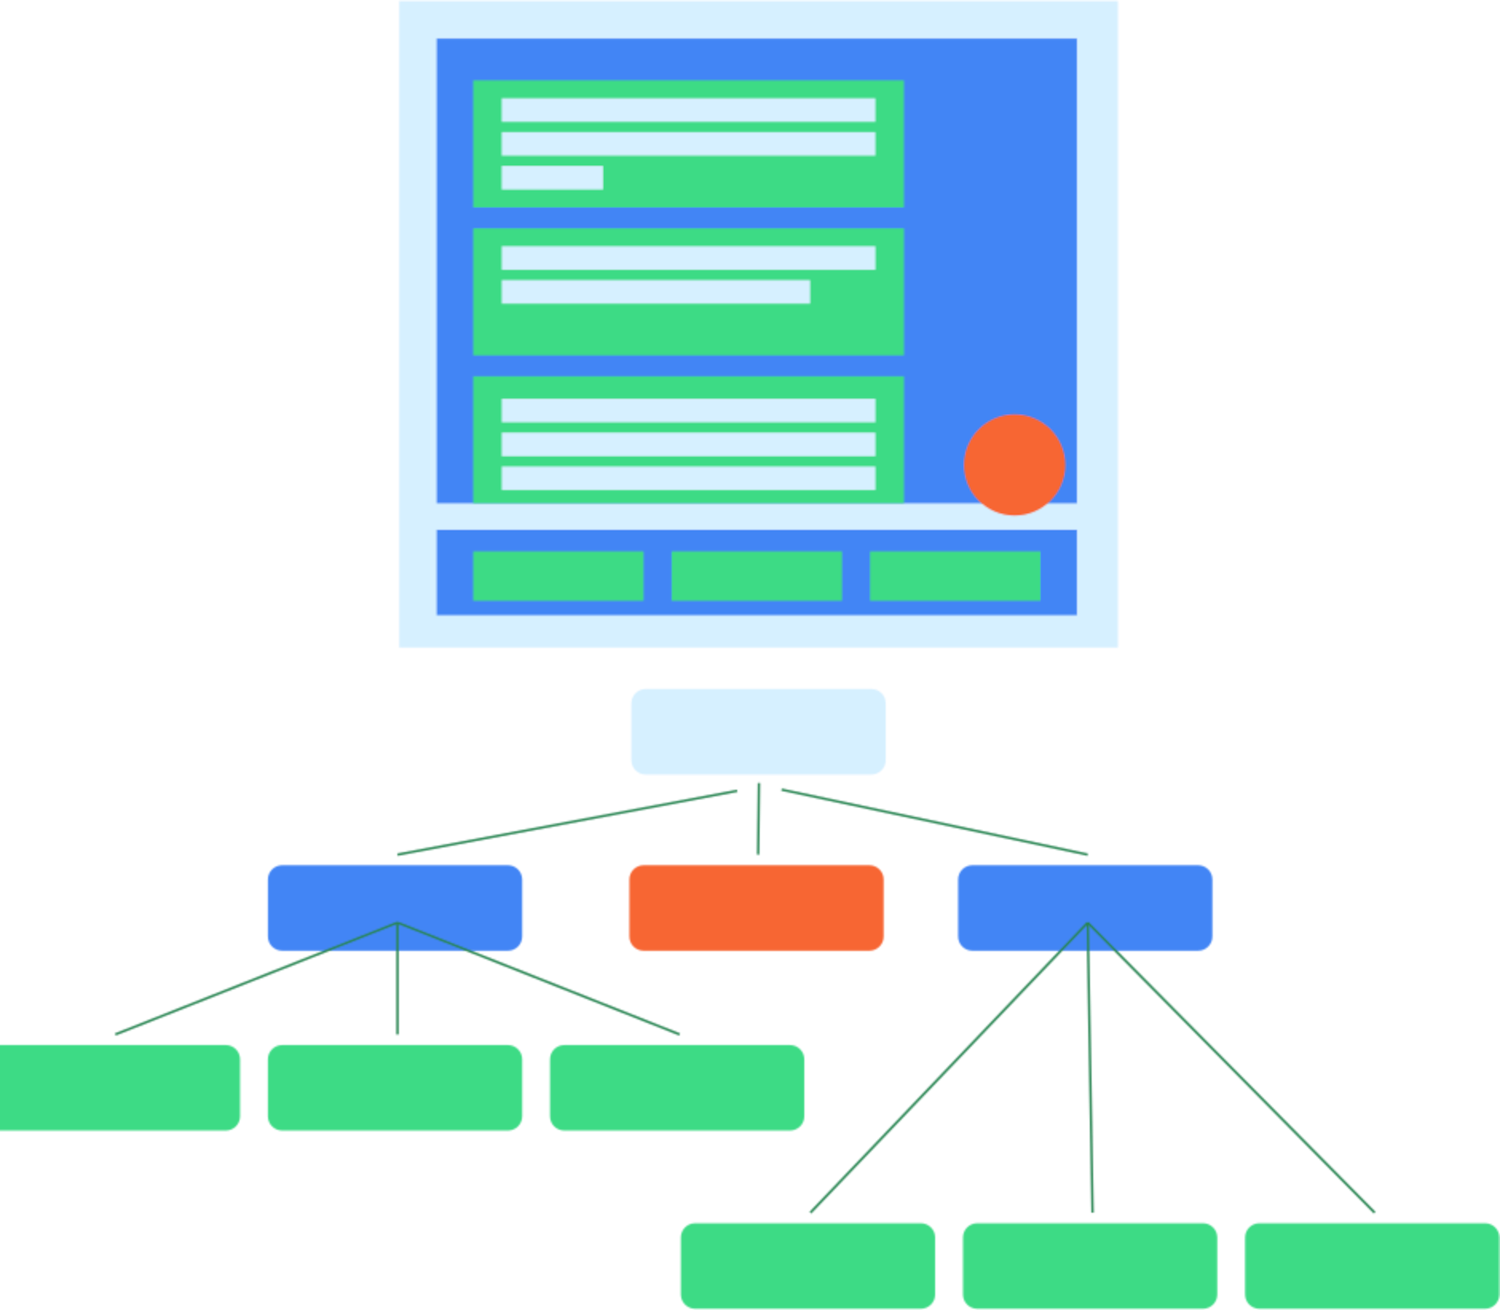
\includegraphics[width=.5\textwidth]{semantics-ui-tree.png}
  \caption{UI struktura a její sémantický strom}
  \label{fig:semantics-ui-tree}
\end{figure}

\myparagraph{Layout}
Během této fáze se jednotlivým komponentám určí na jakých pozicích se mají vykreslit a jakou mají mít šířku a výšku.
Compose během této fáze prochází strom UI komponent tak, že nejprve změří velikost svých potomků (pokud existují) a následně se 
na základě těchto měření rozhodně o vlastní velikosti. Nakonec umístí každého potomka relativně ke své pozici.\cite{jetpackPhases}

Díky použití tohoto algoritmu je k prostupu celého stromu zapotřebí navštívit každý uzel pouze jednou, což je výhodné jelikož
s přibývajícími uzly roste čas potřebný k průchodu celého stromu pouze lineárně. \cite{jetpackPhases}

\myparagraph{Drawing}
V rámci poslední fáze dochází s samotnému vykreslení komponent na obrazovku koncového zařízení. \cite{jetpackPhases}
Compose během této fáze znovu postupně prochází strom UI elementů od kořene až do listů a každý element tohoto stromu vykreslí sám sebe 
na pozici určenou během Layout fáze. \cite{jetpackPhases}

\subsubsection{Kotlin Multiplatform} \label{kmpSection}


%https://blog.jetbrains.com/kotlin/2023/11/kotlin-multiplatform-stable/#use-the-power-of-the-growing-kotlin-multiplatform-ecosystem

Kotlin Multiplatform je často základním kamenem pro tvorbu multiplatformních aplikací založených na Compose Multiplatform a to
z toho důvodu, že díky KMP je možné implementovat multiplatformní aplikační logiku, která může doplňovat multiplatformní UI 
poskytované frameworkem Compose Multiplatform. \cite{KMPUseCases} Důležitým rozdílem oproti ostatním multiplatformním frameworkům 
je právě ta možnost, kterou KMP případně Compose Multiplatform vývojářům poskytuje. 

Jelikož se jedná o SDK, tak umožňuje vývojářům implementovat multiplatformní funkcionality postupně, bez nutnosti implementovat 
v Kotlinu celé vrstvy aplikací. Díky tomu dává vývojářům možnost sdílet napříč platformami je ty části kódu, které mají největších
smysl implementovat pro veškeré platformy a zbylé části kódu psát v nativním jazyce pro danou platformu. \cite{KMP}
Lépe je tato skutečnost ilustrována na následujícím obrázku \ref{fig:KMP_vrstvy}, na kterém jsou vidět různé možnosti,
jakými může být KMP na daných platformách implementován.

\begin{figure}[H]
  \centering
  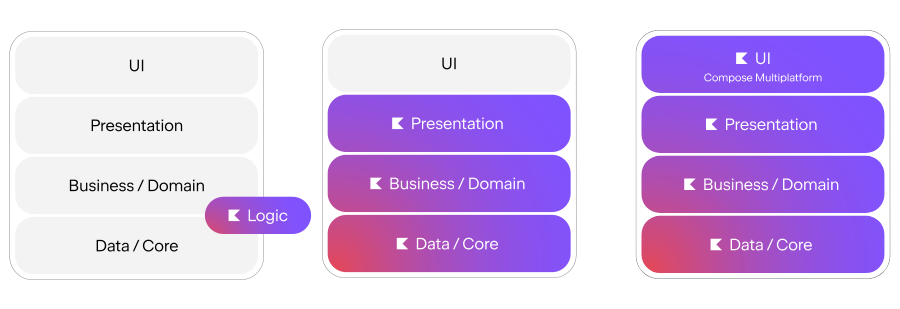
\includegraphics[width=.7\textwidth]{KMP_vrstvy.png}
  \caption{Možnosti implementace KMP}
  \label{fig:KMP_vrstvy}
\end{figure}

Zároveň je tento obrázek ukázkou toho, jak může probíhat migrace z již naimplementované nativní aplikace na aplikaci
multiplatformní. Nejprve je tedy možné implementovat jen malou část aplikační logiky pro víro platforem a postupem času přesouvat
do multiplatformní části aplikace například celé vrstvy starající se o prezentační, datovou nebo jinou aplikační logiku. \cite{KMPUseCases}

Aby ale k takové migraci mohlo dojít, tak je zapotřebí aby pro technologie používané v původní nativní aplikaci existovali multiplatformní
knihovny nebo alespoň jejich ekvivalent.

\subsubsection*{Multiplatformní knihovny}
Společnost JetBrains ve svém článku z konce roku 2023 zmiňuje, že existuje již přes 1500 KMP knihoven s tím, že ještě v roce 2020
jich bylo pouze několik málo desítek. \cite{KMPstable}

%Jeho hlavním úkolem je sdílení kódu na mobilních platformách. 
Právě počet a vyspělost těchto knihoven se podle společností, které již KMP používají jeví jako zatím jedna z nejslabších stránek KMP 
(viz sekce \textit{Aktuální použití KMP v praxi %\ref{kmpInPractise}
}).

V případě, že žádná vhodná knihovna není k dispozici, tak je zde stále možnost čehož je možné docílit díky funkcionalitě jazyka Kotlina
zvané Expected a actual deklarace.

\subsubsection*{Expected a actual deklarace}\label{expectActual}
Deklarace \textit{expected} a \textit{actual} umožňují přistupovat k platformě specifickým API z Kotlin Multiplatform modulů. \cite{KMPExpectActual}
Nejprve je ve společné části potřeba vytvořit například třídu nebo funkci u které chceme aby její obsah byl implementován typicky pomocí
platformě specifických knihoven a tuto část v rámci společného modulu označit klíčovým slovem \code{expect}. \cite{KMPExpectActual} Její implementaci následně provést v rámci
platformě specifického kódu. Tato implementace musí být provedena pod stejným názvem a ve stejném balíku jako deklarace ve společném modulu
a musí být označena klíčovým slovem \code{actual}. \cite{KMPExpectActual}

Během kompilace pak Kotlin kompilátor každou deklaraci s klíčovým slovem \code{expect} sjednotí s příslušnou actual deklarací pro danou platformu
a vygeneruje z ní jednu deklaraci obsahující actual implementaci. \cite{KMPExpectActual}

\subsubsection*{Struktura KMP projektů}\label{projectStructure}
Jak již bylo zmíněno v úvodu, tak jedním z hlavních cílů multiplatformního vývoje je mít 
jeden kód, který by bylo možné zkompilovat tak, aby byl spustitelný je všech požadovaných platformách. To však u KMP není vždy 
možné, a proto je nutné, zvlášť rozdělit kód, který je určen pro všechny platformy a kód, který je platformě specifický. 

\myparagraph{Společný kód}
Jedná se o kód sdílený mezi různými platformami a měl by být seskupen v adresáři \code{commonMain}. \cite{KMPCommonCode}

Kotlin kompilátor na základě zdrojových kódů umístěný v tomto adresáři generuje sadu binárních souborů specifických pro danou platformu. \cite{KMPCommonCode}
Při kompilaci tak může z téhož kódu vygenerovat několik souborů, jako například soubory pro \textit{Java Virtual Machine (JVM)}, 
anebo spustitelné soubory pro nativní platformu. \cite{KMPCommonCode}

Nicméně i pro jednotlivé platformy existují zařízení, která například využívají specifickou architekturu, a proto je třeba pro 
tato zařízení zkompilovat tento kód jiným způsobem.

K této kompilaci KMP používá technologii Kotlin/Native, díky které
je možné sestavovat kód napsaný v jazyce Kotlin do nativních binárních souborů a ten díky tomu může běžet i bez JVM. \cite{kotlinNative}

Pro ukázku toho, jaká zařízení jsou technologií Kotlin/Native podporovaná slouží následují obrázek \ref{fig:KMP_struktura}

\begin{figure}[H]
  \centering
  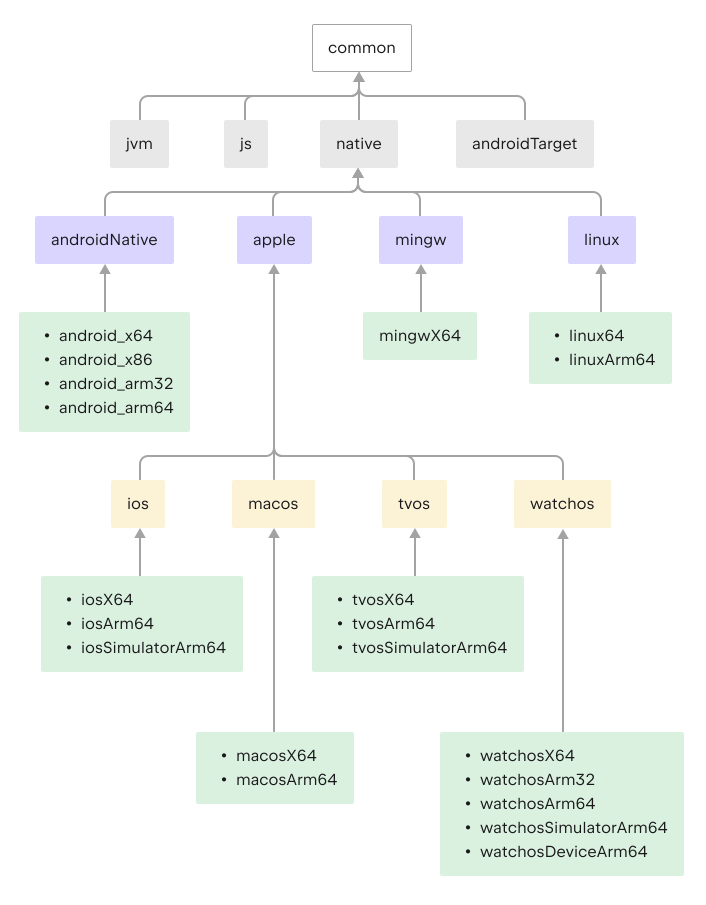
\includegraphics[width=.7\textwidth]{full-template-hierarchy.png}
  \caption{Hierarchická struktura KMP \cite{KMPHierarchi}}
  \label{fig:KMP_struktura}
\end{figure}

Při této vizualizaci veškerých podporovaných zařízeních se ale ukazuje, že rozřazení kódu do vhodných balíčků je pro orientaci v 
multiplatformním projektu založeném na KMP klíčové. Implementace kódu pro každé jednotlivé zařízení by byla zbytečná, jelikož
velké části kódu i těchto platformě specifických kódu mohou být součástí společného kódu. Nesdílení toho kódu s ostatními platformami
by tak zapříčinilo duplikaci velké části kódu. 

Aby se tomuto zabránilo je vhodné využít dříve zmíněné hierarchické struktury a využít takzvané \textit{source sets}, které slouží 
pro jakési seskupení kódů specifických pro konkrétní zařízení nebo platformy. Pro lepší představu o tom jak jsou jednotlivé
\textit{source sets} definovány slouží obrázek \ref{fig:dependson-tree-diagram},
který vizualizuje celkem pět zadefinovaných \textit{source sets} a to konkrétně \code{commonMain}, \code{androidMain}, 
\code{iosMain}, \code{iosSimulatorArm64} a \code{iosArm64}. V rámci těchto zdrojových sad mohou být následně implementovány
platformě specifické knihovny čemuž se detailněji věnuje kapitola \textit{Gradle \ref{gradleChapter}} v implementační části práce.

%pro které může být například použit specifický kód nebo 
%Díky nim je možné sdílet společný kód pouze mezi některými podporovanými platformami. \cite{KMPHierarchi}
%%. Pomocí nich je možné sestavovat 
%projekt pro vícero zařízení zároveň.

\begin{figure}[H]
  \centering
  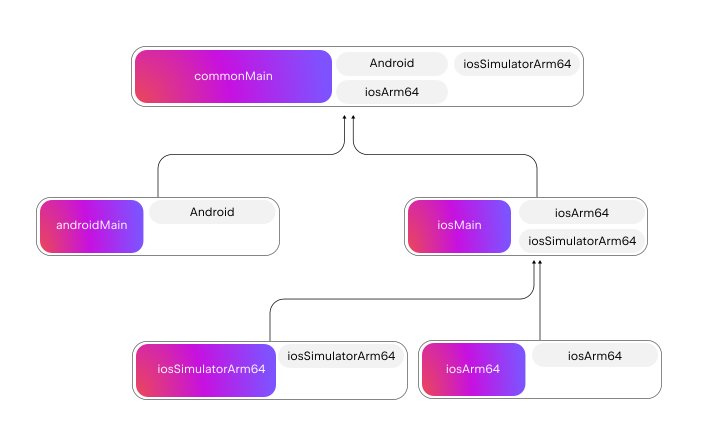
\includegraphics[width=.9\textwidth]{dependson-tree-diagram.png}
  \caption{Strom závislostí}
  \label{fig:dependson-tree-diagram}
\end{figure}

Ze struktury těchto zdrojových sad zároveň vyplývá koncová struktura projektu, která se ve většině případů obsahuje adresář pro sdílený kód (\code{commonMain}), 
který smí obsahovat pouze kód a případné knihovny, které jsou multiplatformní a pokrývají tak veškeré platformy používané v projektu.

A dále na adresáře pro vybrané platformy jako například \code{AndroidMain}, \code{iosMain}, které již mohou být závislé na pouze platformě specifický knihovnách.

\subsubsection*{Aktuální použití KMP v praxi} \label{kmpInPractise}
% Mezi další důvody patří taktéž lepší zastupitelnost jednotlivých členů týmu a to díky me

I přesto, že je KMP ve stabilní verzi teprve od listopadu 2023 \cite{KMPstable}, tak tuto technologii používá již několik světově 
známých firem v produkčním nasazení jako je například Forbes či McDonald's. Forbes uvádí, že právě díky KMP dokáží sdílet až 80 \%
aplikační logiky napříč platformami Android a iOS. \cite{KMPinForbes} 
Druhý ze jmenovaných McDonald's jako hlavní výhody uvádí jednodušší testování \cite{KMPinMcDonalds}

Naopak mezi největší výzvy, které obě společnosti ve svých souhrnech uvádějí patří adaptace na KMP prostředí (především iOS vývojářů) nebo
nedostatečné množství potřebných multiplatformních knihoven (případně jejich nedostatečná vyspělost). \cite{KMPinForbes} \cite{KMPinMcDonalds}

Pro porovnání s 

\emph{"Od této doby jsme vyvinuli a v produkci provozujeme několik mobilních aplikací. Ze zkušenosti vidíme, že při jejich vývoji dokážeme 
sdílet cca 60–70 \% kódu na platformu. V případě vývoje na dvě platformy to znamená, že v součtu dokážeme ušetřit minimálně třetinu 
nákladů na vývoj, plus s tím související další náklady na věci typu testování (v tomto případě snížení až na polovinu)."}

\begin{figure}[H]
  \centering
  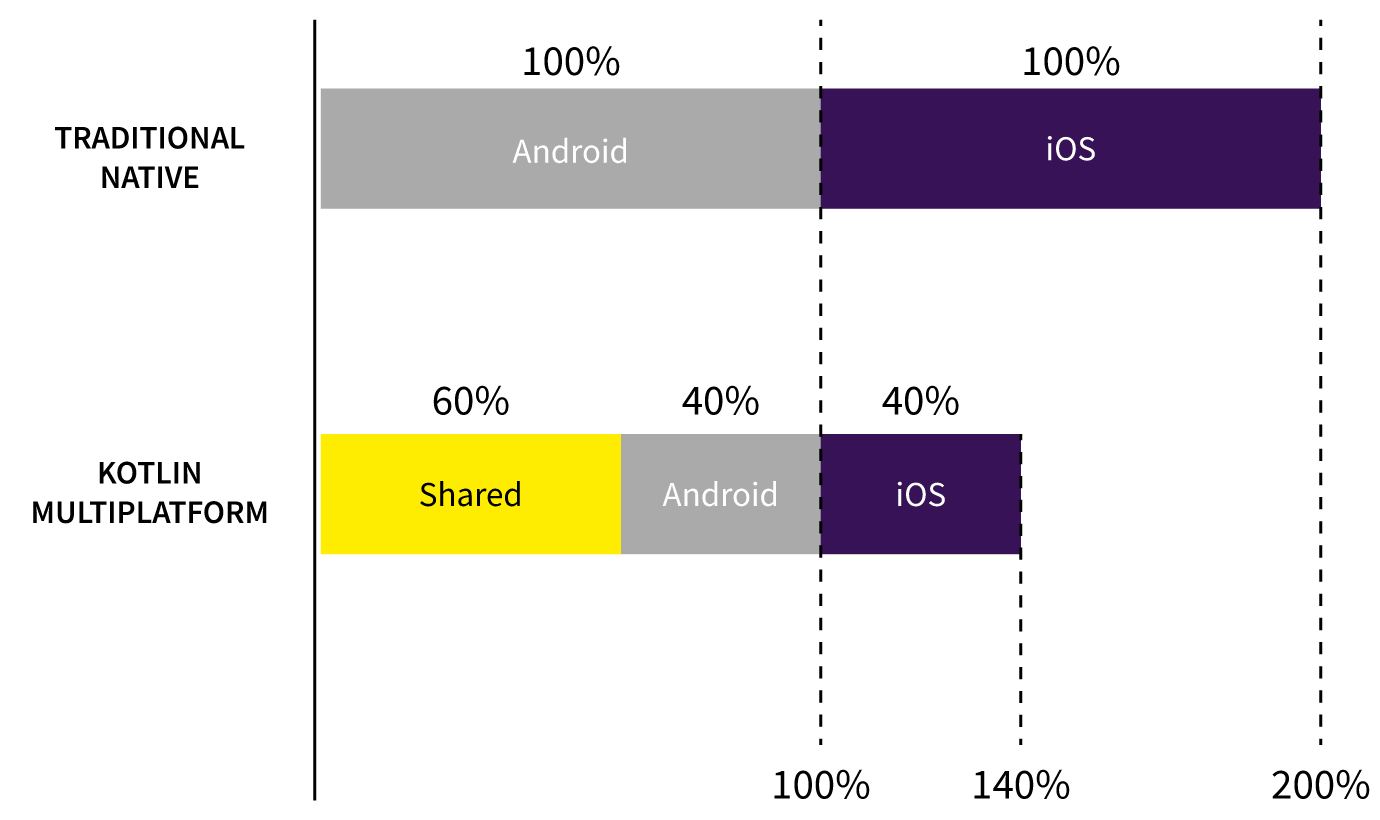
\includegraphics[width=.55\textwidth]{chart-KMP-vs-native.png}
  \caption{Množství kódu KMP vs native}
  \label{fig:KMP_vs_native}
\end{figure}

Pro upřesnění je ještě potřeba zmínit, že veškeré vyjmenované společnosti, využili pouze možnosti sdílení logiky a nepoužívají
tak sdílené UI pomocí Compose Multiplatform.

To se ukázalo i na průzkumu, který provedla společnost JetBrains v roce 2021, kde pouze 3,8~\% respondentů odpovědělo, že byli schopni sdílet UI ve svých aplikacích.

Pro ukázku veškerých částí, které respondenti sdíleli ve svých aplikacích napříč platformami slouží obrázek \ref{fig:KMPSurvey}, který jednoznačně ukazuje, že
mezi nejčastěji sdílené části aplikací patří datová a síťová vrstva.  

\begin{figure}[H]
  \centering
  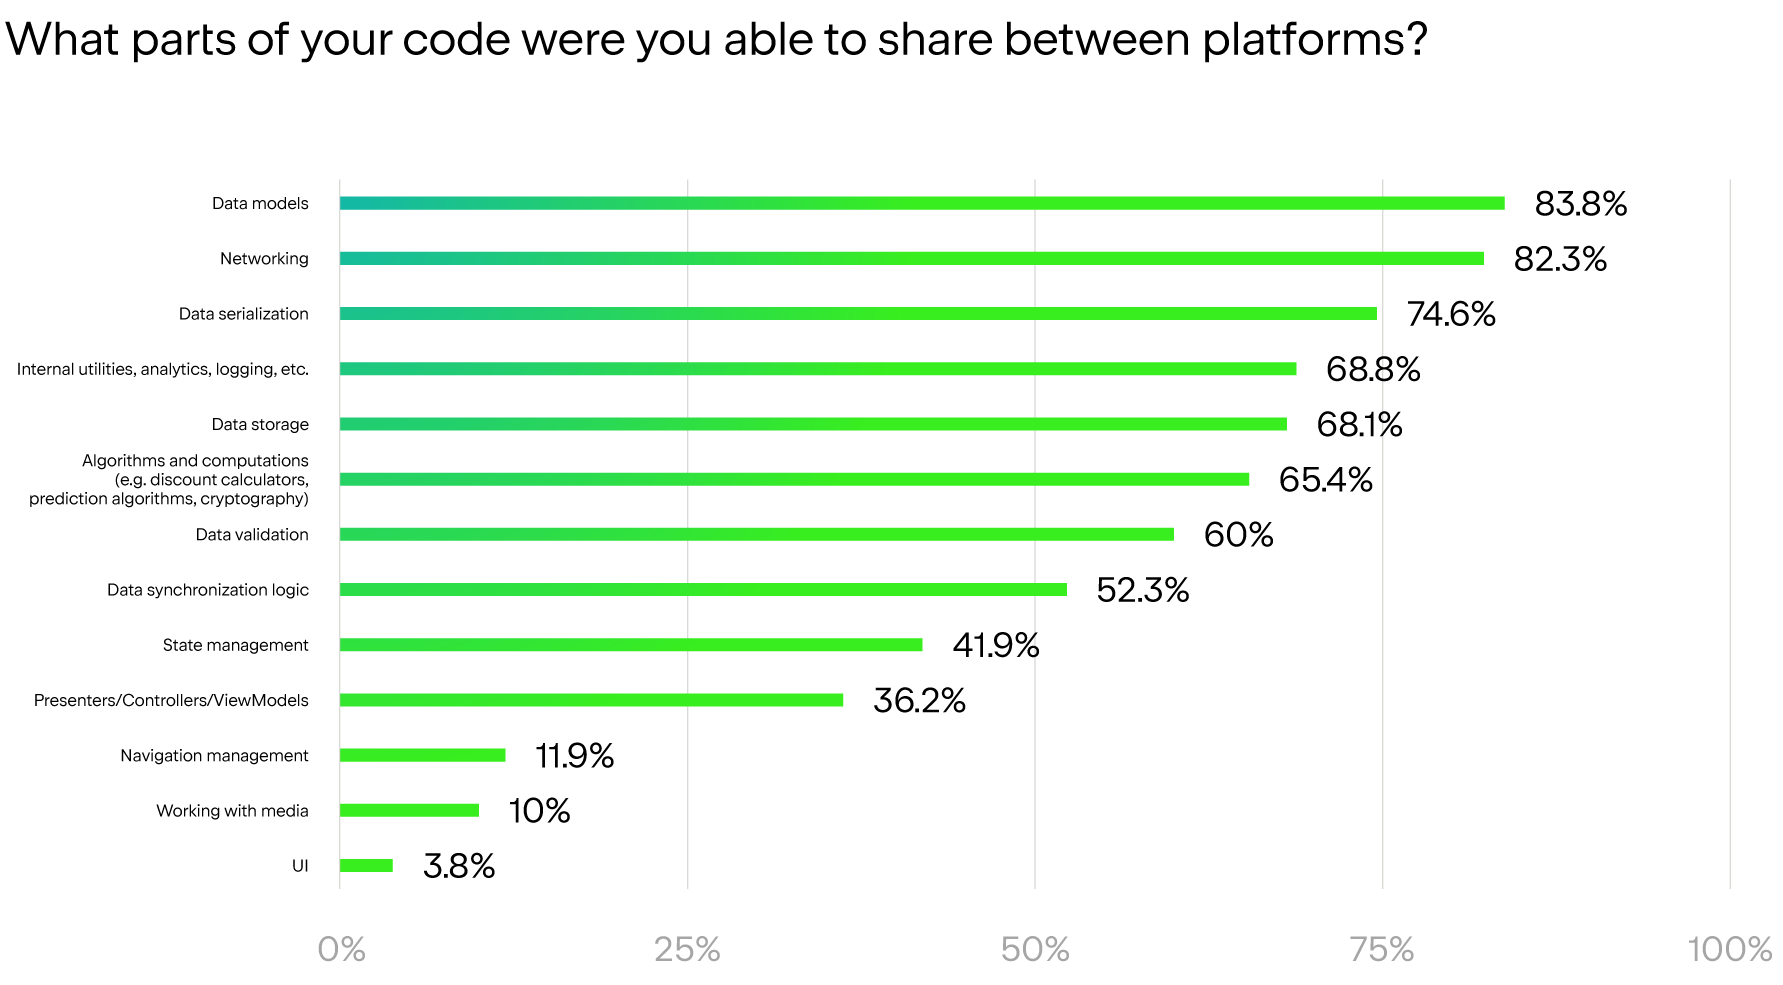
\includegraphics[width=1\textwidth]{survey-results-q1-q2-22-light.png}
  \caption{KMP průzkum}
  \label{fig:KMPSurvey}
\end{figure}

\section{Porovnání vybraných multiplatformních frameworků}

V rámci této kapitoly budou porovnány vybrané multiplatformní frameworky


\subsection{Porovnání výkonu}

Mezi klíčové parametry, kvůli kterým většina firem upřednostňuje vývoj nativních aplikací, patří především výkon
nativních aplikací. Z toho důvodu se následující podkapitola věnuje právě porovnání výkonu a dalších parametrů multiplatformních aplikací s
nativními verzemi aplikací. 

Pro testování byly použity toolkity pro tvorbu nativního UI pro platformu Android (Jetpack Compose) a iOS (SwiftUI)
v porovnání s multiplatformním frameworkem Compose Multiplatform a aktuálně nejpoužívanějším multiplatformním
frameworkem zvaném Flutter. \cite{crossPlatformFrameworksStats} 

Mezi hlavní testované parametry patřil čas nastartování testované aplikace a její velikost.

\subsection*{Ukázková aplikace}
Pro porovnání důležitých parametrů byla pro test vytvořena jednoduchá aplikace, která obsahovala jednu obrazovku, 
načetla obrázky z veřejného API a zobrazila je v horizontálním seznamu. 
Na každý obrázek šlo kliknout a zobrazit jej přiblížený pod seznamem. 

Veškeré testy proběhli na zařízeních Pixel 4a a iPhone 12 Mini a byly opakovány celkem pětkrát.

%Verze Compose Multiplatform 1.4

% replikovat test


\myparagraph{Velikost aplikace} 

Na obrázku \ref{fig:chart_app_sizes} je vidět, že velikost aplikace založené na Compose Multiplatform je identická
s velikostí nativní aplikace pro Android. Je tomu tak z toho důvodu, že výsledná aplikace pro Android neobsahuje kód 
pro jiné platformy. \cite{} Kdežto u velikosti iOS aplikace je situace výrazně jiná. Samotná aplikace pro iOS je v porovnání
s její nativní aplikací o 23,1 MB větší. Tento rozdíl ve velikosti je způsoben především grafickou 2D knihovnou Skia,
která je na platformě Android dostupná, kdežto na platformě iOS ne a proto tam musí být spolu s aplikací dodána. \cite{}

Zajímavé je následné porovnání s velikostí aplikace založené na frameworku Flutter, jelikož ta, stejně jako Compose
Multiplatform využívá knihovnu Skia, ale i přesto je o něco menší než Compose Multiplatform aplikace na platformě iOS.
Součástí aplikace Flutter ještě vlastní engine, který je součástí aplikace a zvětšuje tak velikost aplikace asi o 3–4 MB pro Android a 10 MB 
pro iOS. \cite{flutterSize}

\begin{figure}[H]
  \centering
  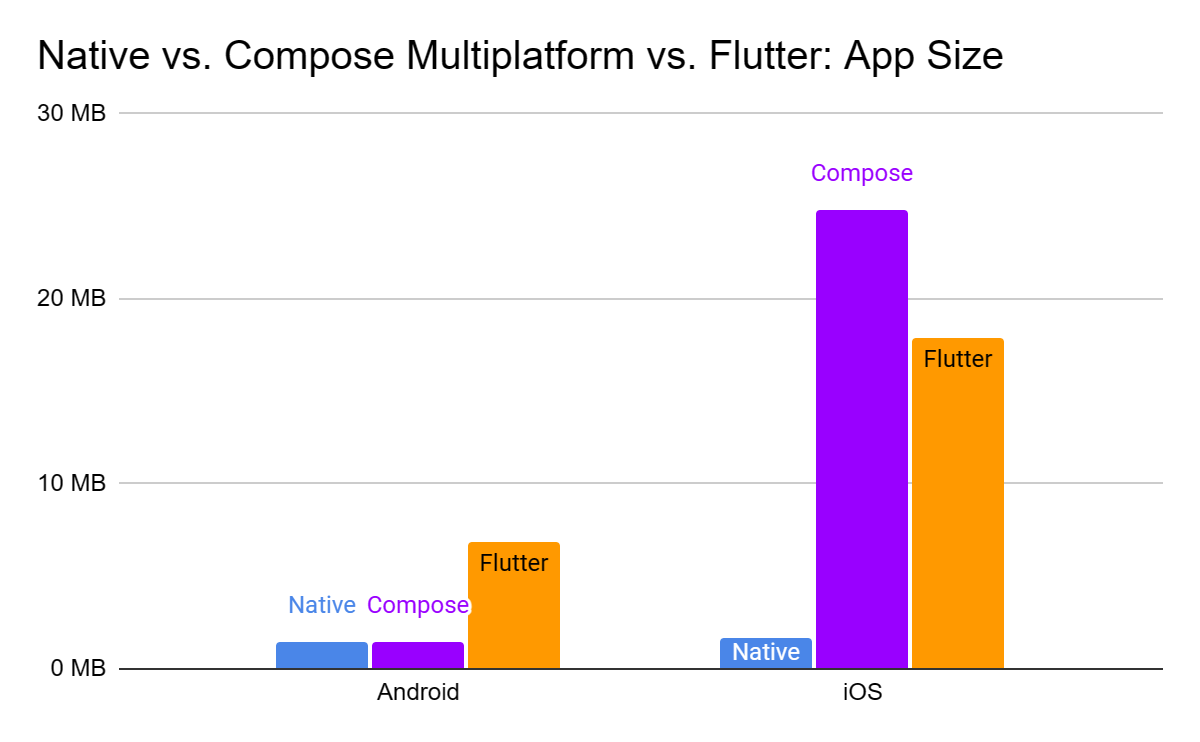
\includegraphics[width=.7\textwidth]{chart_app_sizes.png}
  \caption{APK/IPA size in megabytes}
  \label{fig:chart_app_sizes}
\end{figure}

\myparagraph{Rychlost spuštění aplikace}

Při porovnání rychlosti spuštění Compose Multiplatform aplikace na platformě Android není mezi rychlostmi téměř žádný
rozdíl stejně tak jako tomu při porovnání velikosti aplikací v předchozí kapitole. O něco delší dobu spuštění měla
aplikace napsaná pomocí frameworku Flutter, která se spouštěla v průměru o 221 ms déle než Compose Multiplatform aplikace. 
Toto zpomalení je s nejvyšší pravděpodobností způsobeno dobou spuštění Flutter Enginu, což by korespondovalo s oficiální
Flutter dokumentací. \cite{flutterPerformance}

U posledního porovnání na platformě iOS se doba spuštění aplikací založených na Compose Multiplatform a frameworku 
Flutter o tolik nelišila od nativní aplikace.
% // TODO posledni cast porovnani

% // TODO posledni tabulka pro porovnani https://github.com/jacobras/flutter-vs-native-vs-kmp

\begin{table}[H]
  \centering
  \caption{Porovnání rychlosti spuštění ukázkové aplikace na platformě Android}
  \begin{tabular}{|l|c|c|c|}
    \hline
       & min. & median & max. \\ \hline 
      Native Android & 408.7 ms & 413.1 ms & 423.1 ms \\
      KMP Android & 403.6 ms & 425.3 ms & 466.4 ms \\
      Flutter Android & 600.5 ms & 634.2 ms & 649.8 ms \\ \hline
  \end{tabular}
  \label{tab:performance_comparison}
\end{table}

\begin{table}[H]
  \centering
  \caption{Porovnání rychlosti spuštění ukázkové aplikace na platformě iOS}
  \begin{tabular}{|l|c|}
      \hline
       & Duration (AppLaunch) \\
      \hline
      Native iOS & 1.441 s \\
      KMP iOS & 1.618 s \\
      Flutter iOS & 1.608 s \\
      \hline
  \end{tabular}
  \label{tab:app_launch_duration_ios}
\end{table}


\begin{figure}[H]
  \centering
  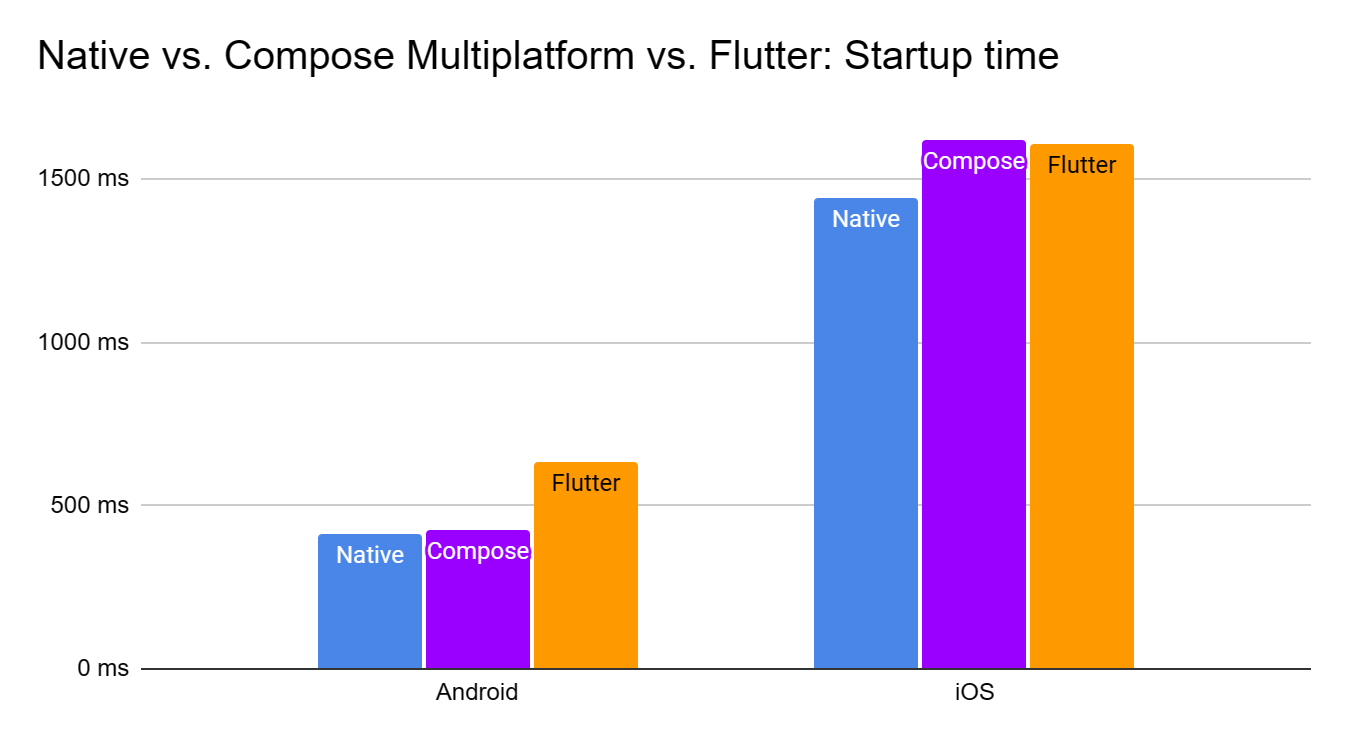
\includegraphics[width=.7\textwidth]{chart_startup_times.png}
  \caption{Časy nastartování jednotlivých aplikací}
  \label{fig:chart_startup_times}
\end{figure}

\subsection{Náročnost implementace}
I přesto, že je náročnost implementace do jisté míry subjektivní záležitostí, tak existuje několik aspektů, které mohou k porovnání 
náročnosti implementace Compose Multiplatform s ostatními frameworky posloužit. 

TODO

\section{Limitace Compose Multiplatform oproti nativnímu řešení} 
% to se tyka KMP ne compose Multiplatform
Jak již bylo zmíněno v kapitole \textit{Kotlin Multiplatform \ref{kmpSection}}, tak jedním z největších problému multiplatformního vývoje pomocí KMP je
především nedostatečné množství knihoven. 

Co se týče UI, tak zde je situace díky možnosti využití Jetpack Compose o něco lepší. Většina omezení, která jsou
aktuálně spjata s UI se týká především plynulosti a nebo použití nativně vypadajících komponent na platformě iOS.
Ta v její nativní podobě používá styl zvaný Cupertino, který frameworkem Compose Multiplatform není aktuálně oficiálně podporován. 
Co se týče plynulosti UI na platformě iOS, tak aktuálně se nejvíce řeší problém s rychlostí vykreslování.

Většina výše zmíněných problémů se již řeší a je zmíněna v Kotlin Multiplatform vývojářském plánu pro rok 2024. \cite{KMPRoaddMap} Konkrétně
se jedná o veškeré zmíněné o problémy kromě zařazení HarmonyOS mezi podporované platformy.% // todo 
V tomto plánu je mimo jiné uvedeno, že aktuální prioritu číslo jedna je dostání frameworku Compose Multiplatform na platformě iOS do verze Beta. \cite{KMPRoaddMap}
